\documentclass[a4paper,12pt]{article}
\usepackage{amsmath}
\usepackage{hyperref}
 \usepackage{graphicx}
 \usepackage{float}
 \usepackage{subcaption}
 \usepackage{listings}

\begin{document}

\title{Spectral Analysis of Convolution with a Rectangular Kernel}
\author{Group Quiz 02 - EE1060}
\date{Spring 2025}
\maketitle

\section*{Spectral Analysis of convolution of $h(t)$ with various $f(t)$}
\subsection*{Trigonometric Functions}
\begin{figure}[H]
    \centering
    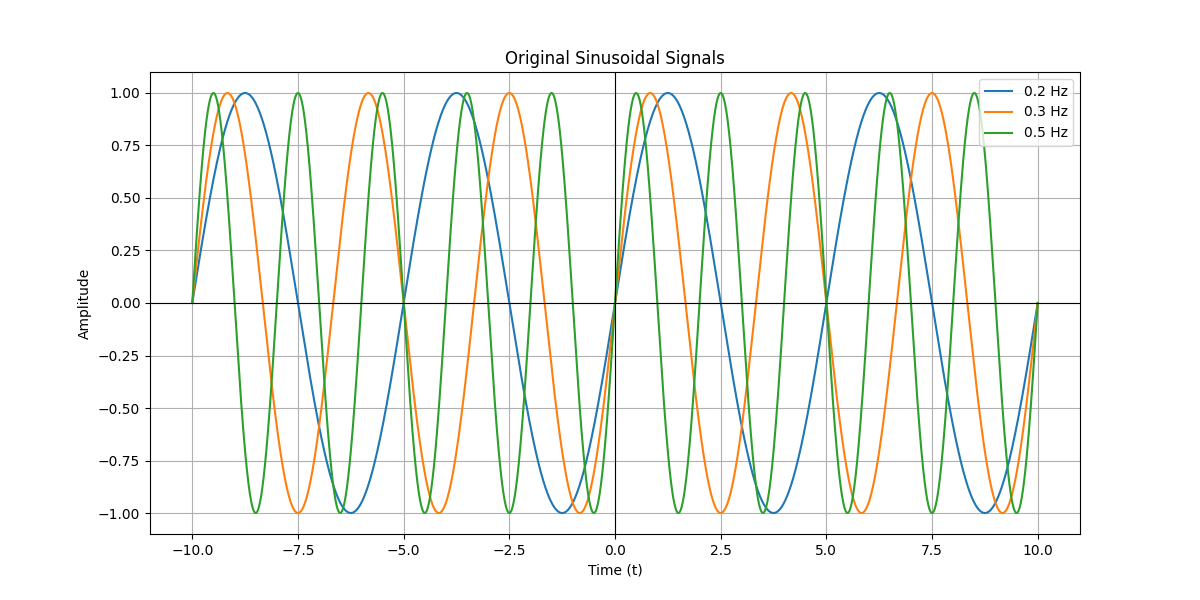
\includegraphics[width=0.7\textwidth]{figs/sin1.png}
\end{figure}
\begin{figure}[H]
    \centering
    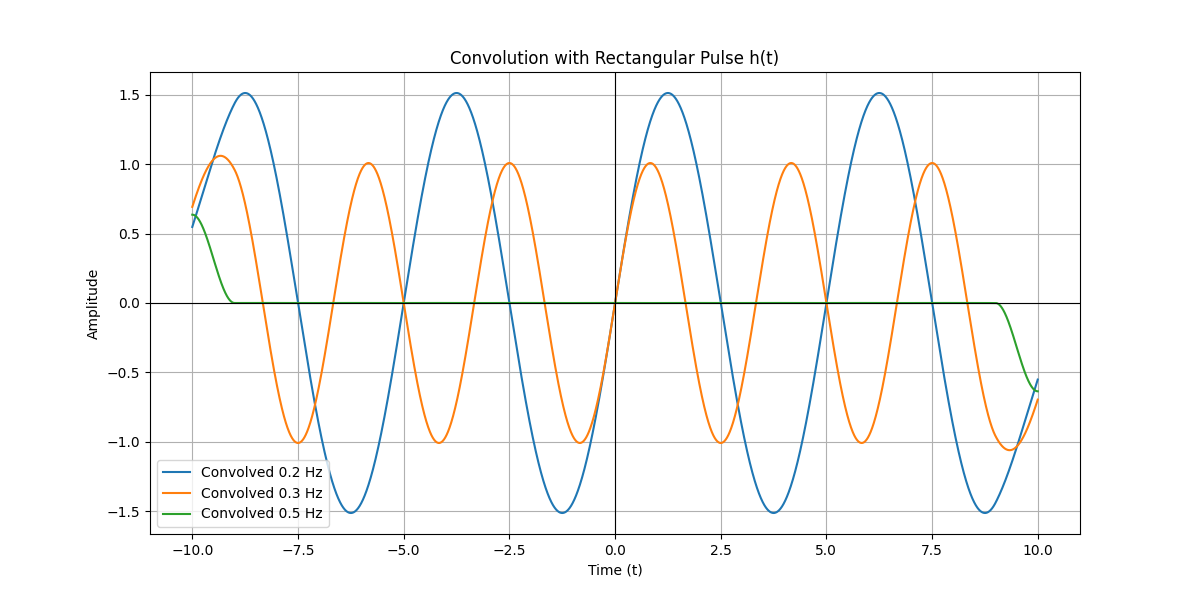
\includegraphics[width=0.7\textwidth]{figs/sin2.png}
\end{figure}
\begin{figure}[H]
    \centering
    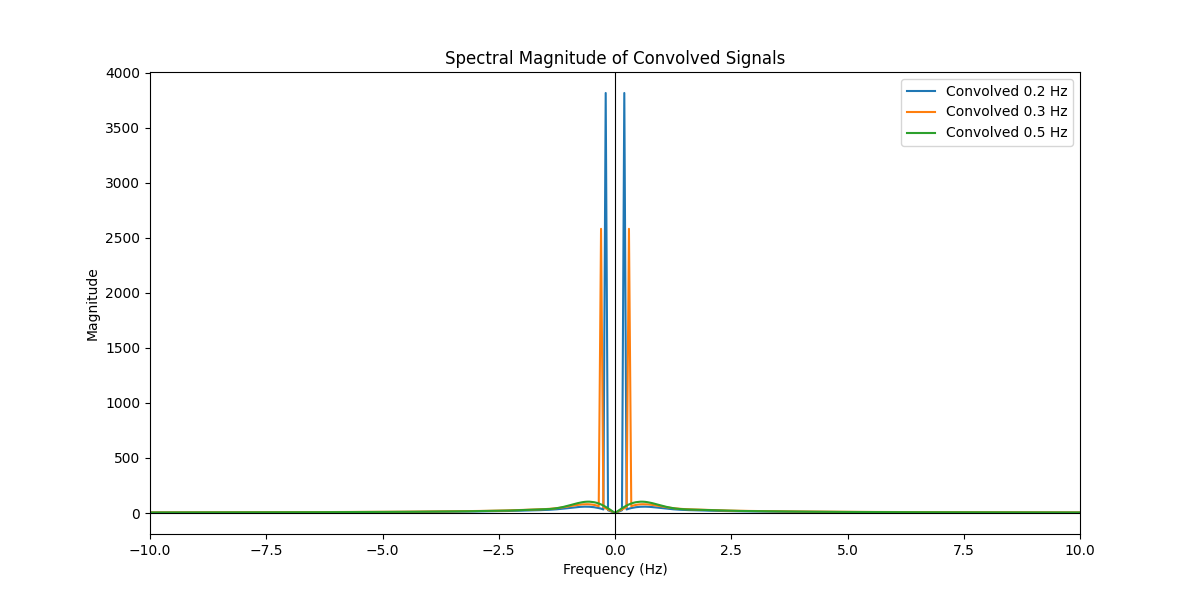
\includegraphics[width=0.7\textwidth]{figs/sin3.png}
\end{figure}
\begin{figure}[H]
    \centering
    \begin{subfigure}{0.5\textwidth}
        \centering
        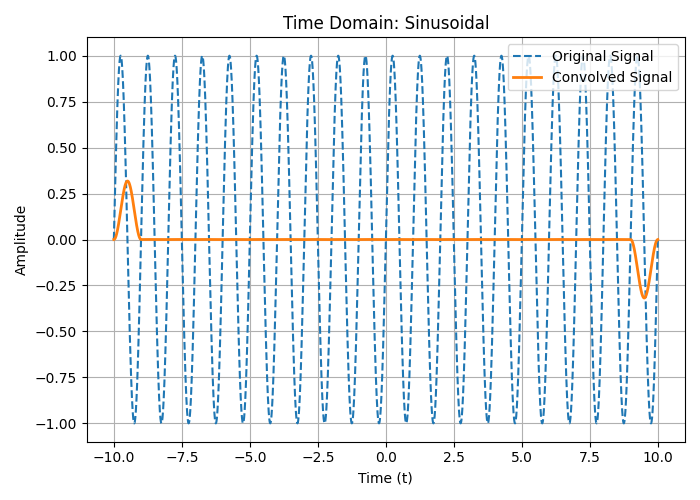
\includegraphics[height=5cm]{figs/Analysis0.png}
    \end{subfigure}%
    \begin{subfigure}{0.5\textwidth}
        \centering
        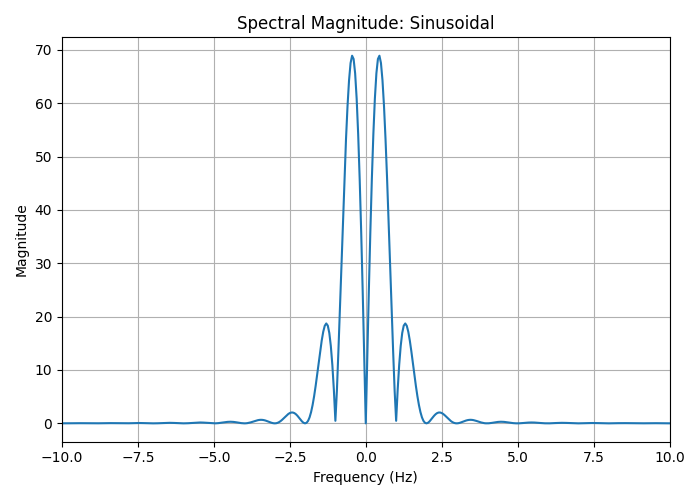
\includegraphics[height=5cm]{figs/Analysis1.png}
    \end{subfigure}
\end{figure}

The rectangular kernel acts as a low-pass filter by scaling the amplitudes of higher frequencies in convolution. Peaks in the spectral analysis plot can be seen at frequencies of the trigonometric functions as they oscillate with that frequency.
\subsection * {Algebraic functions}
\begin{figure}[H]
    \centering
    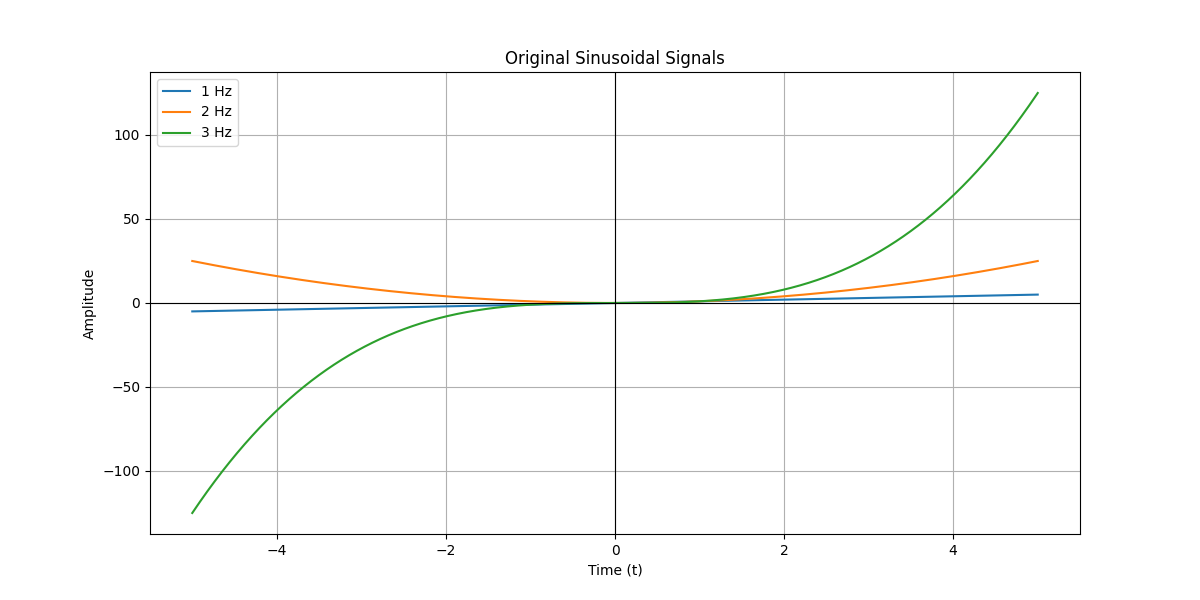
\includegraphics[width=0.7\textwidth]{figs/alg1.png}
\end{figure}
\begin{figure}[H]
    \centering
    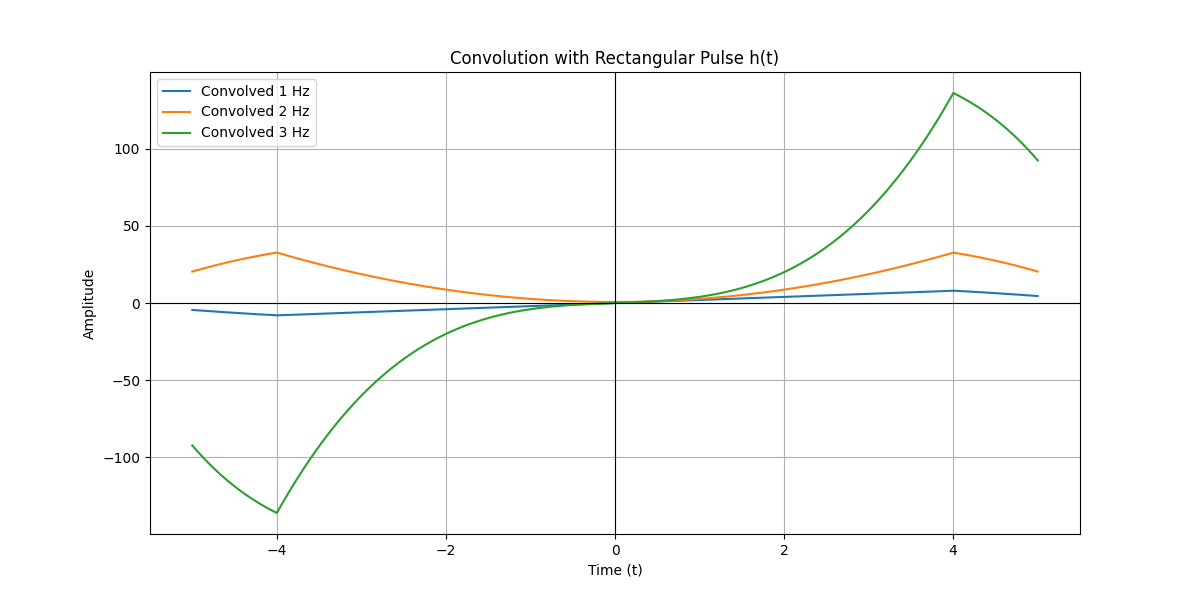
\includegraphics[width=0.7\textwidth]{figs/alg2.png}
\end{figure}
\begin{figure}[H]
    \centering
    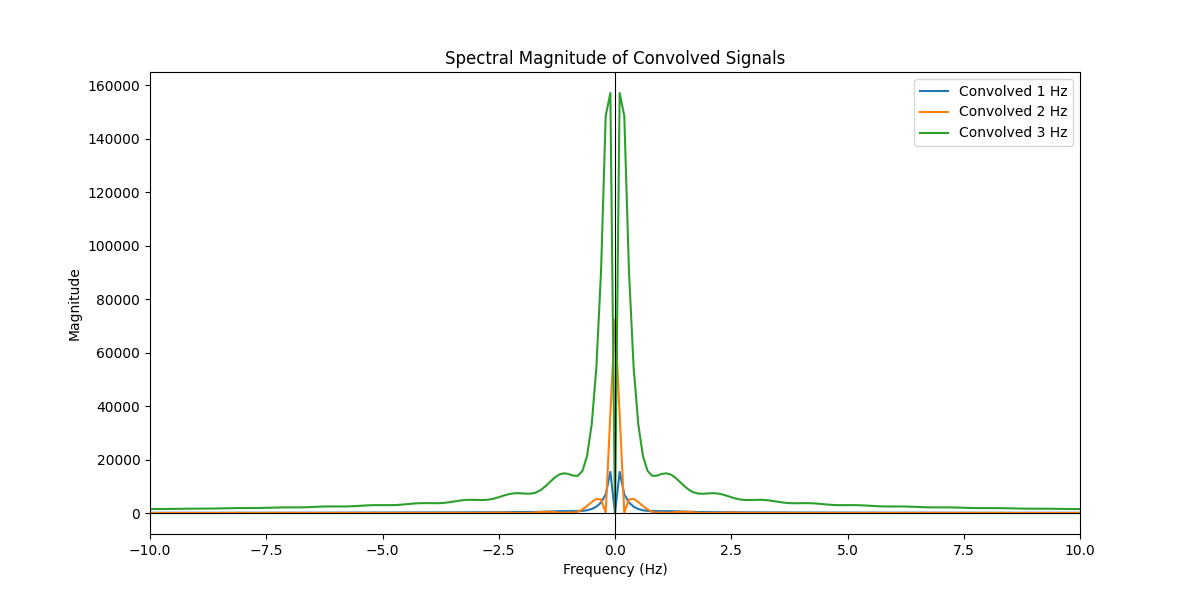
\includegraphics[width=0.7\textwidth]{figs/alg3.png}
\end{figure}
\begin{figure}[H]
    \centering
    \begin{subfigure}{0.5\textwidth}
        \centering
        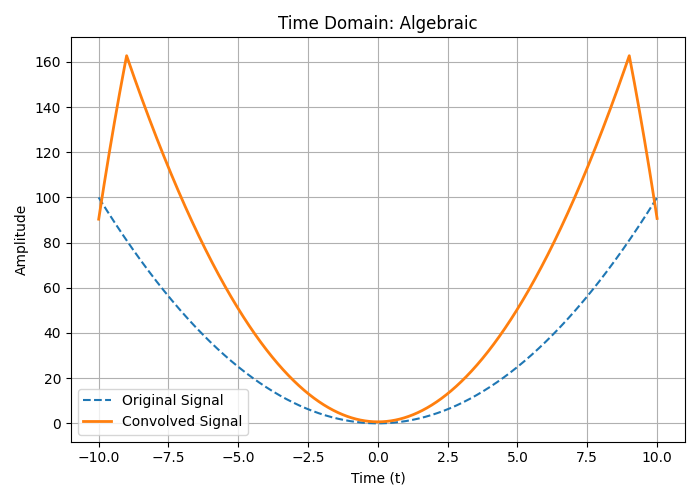
\includegraphics[height=5cm]{figs/Analysis2.png}
    \end{subfigure}%
    \begin{subfigure}{0.5\textwidth}
        \centering
        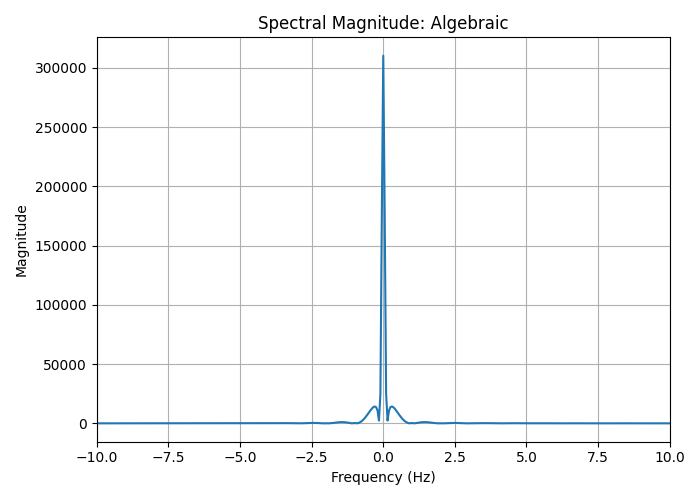
\includegraphics[height=5cm]{figs/Analysis3.png}
    \end{subfigure}
\end{figure}
Peak in spectral Analysis can be seen at frequency=0 as no oscillation
\subsection*{Exponential Functions}
\begin{figure}[H]
    \centering
    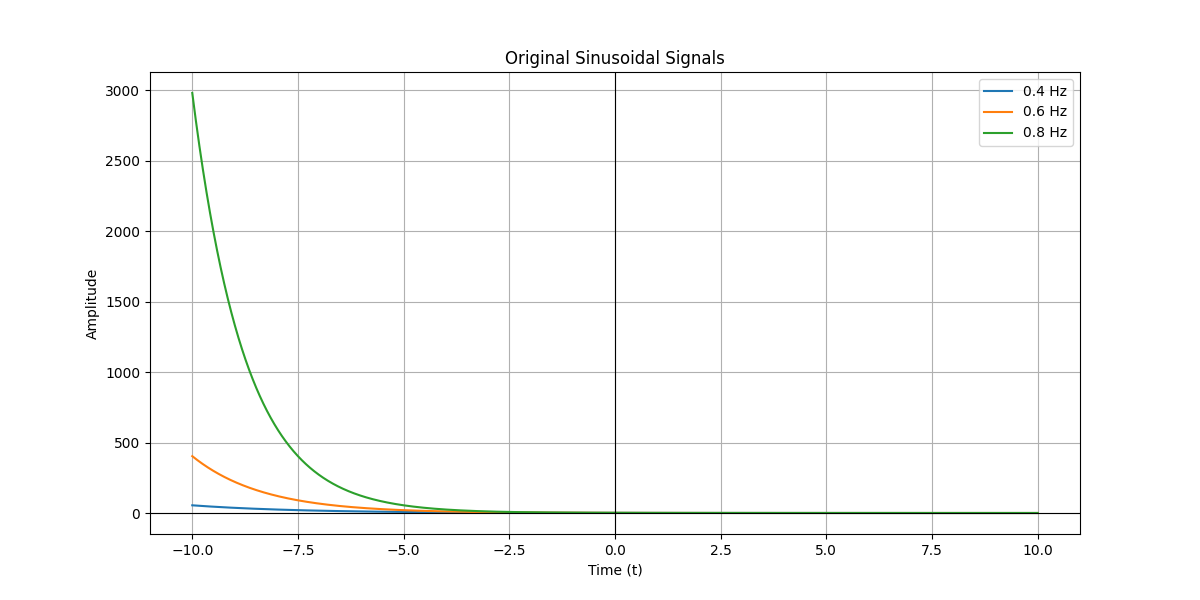
\includegraphics[width=0.7\textwidth]{figs/exp1.png}
\end{figure}
\begin{figure}[H]
    \centering
    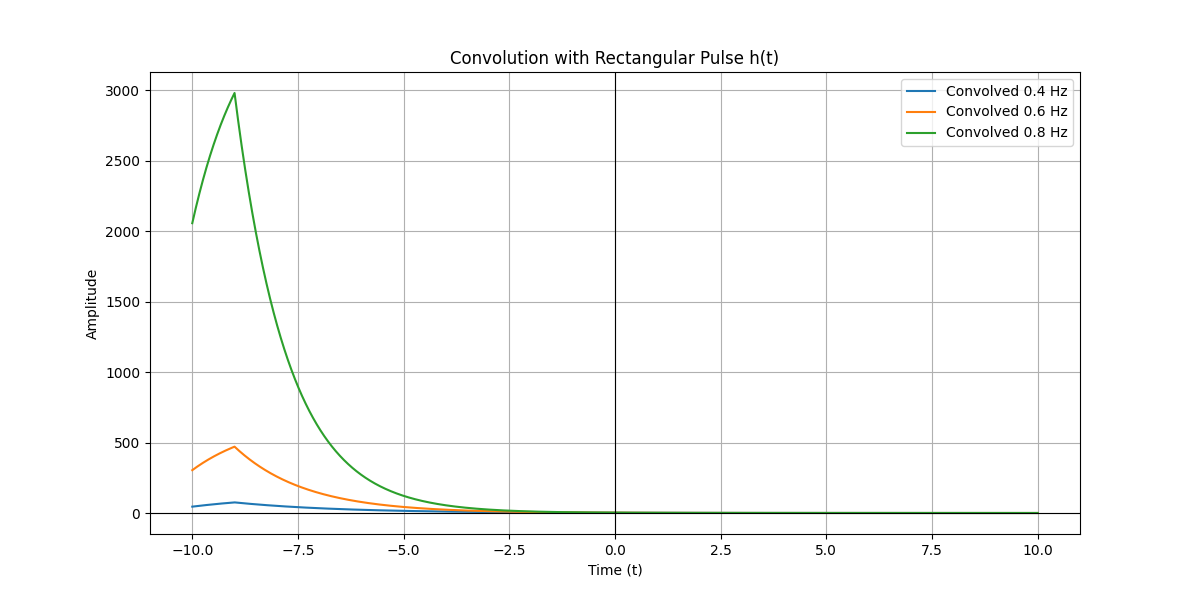
\includegraphics[width=0.7\textwidth]{figs/exp2.png}
\end{figure}
\begin{figure}[H]
    \centering
    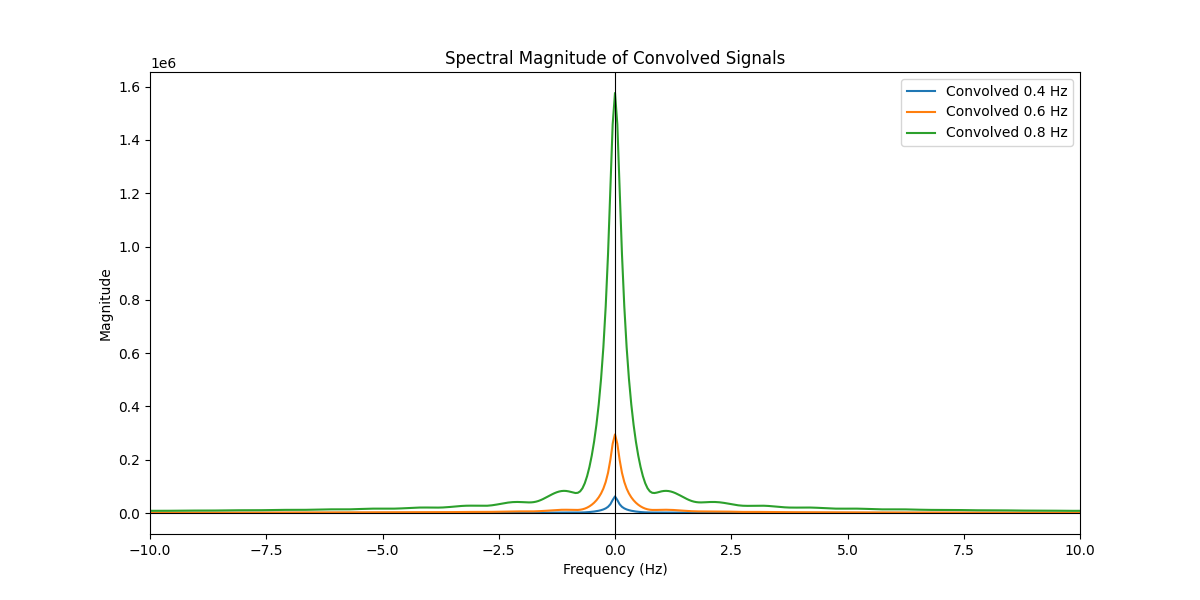
\includegraphics[width=0.7\textwidth]{figs/exp3.png}
\end{figure}
\begin{figure}[H]
    \centering
    \begin{subfigure}{0.5\textwidth}
        \centering
        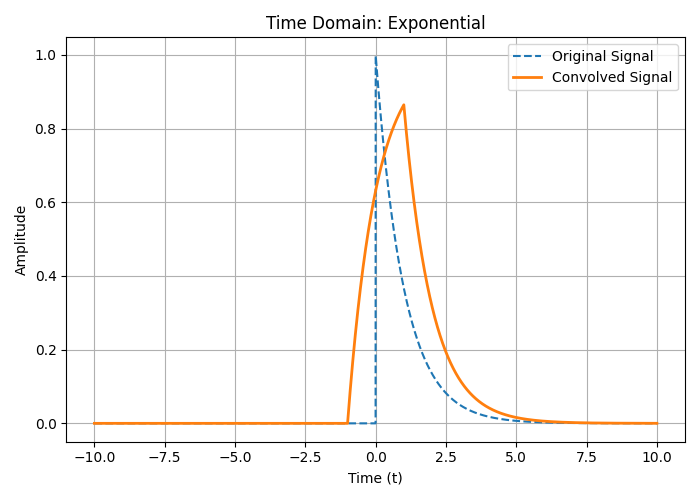
\includegraphics[height=5cm]{figs/Analysis4.png}
    \end{subfigure}%
    \begin{subfigure}{0.5\textwidth}
        \centering
        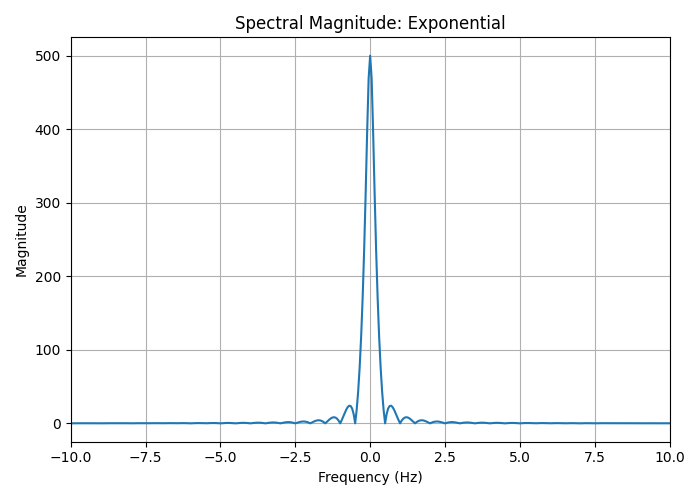
\includegraphics[height=5cm]{figs/Analysis5.png}
    \end{subfigure}
\end{figure}
Peak in spectral Analysis can be seen at frequency=0 as no oscillation
\subsection*{Logarithmic Functions}
\begin{figure}[H]
    \centering
    \begin{subfigure}{0.5\textwidth}
        \centering
        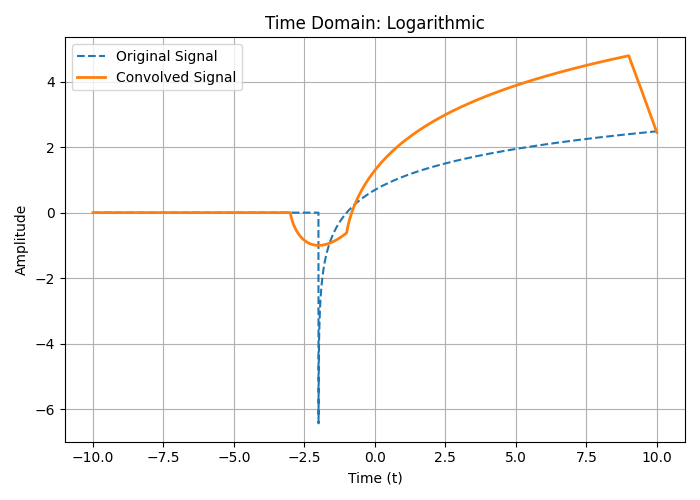
\includegraphics[height=5cm]{figs/Analysis6.png}
    \end{subfigure}%
    \begin{subfigure}{0.5\textwidth}
        \centering
        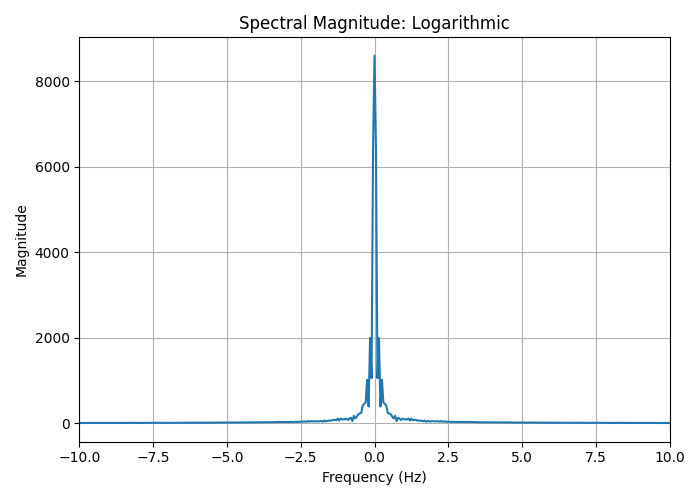
\includegraphics[height=5cm]{figs/Analysis7.png}
    \end{subfigure}
\end{figure}
Peak in spectral Analysis can be seen at frequency=0 as no oscillation
\subsection*{Inverse Tigonomentric Functions}
\begin{figure}[H]
    \centering
    \begin{subfigure}{0.5\textwidth}
        \centering
        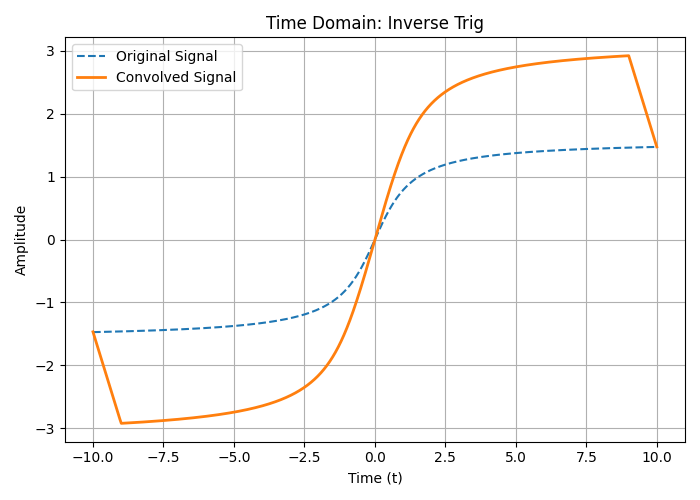
\includegraphics[height=5cm]{figs/Analysis8.png}
    \end{subfigure}%
    \begin{subfigure}{0.5\textwidth}
        \centering
        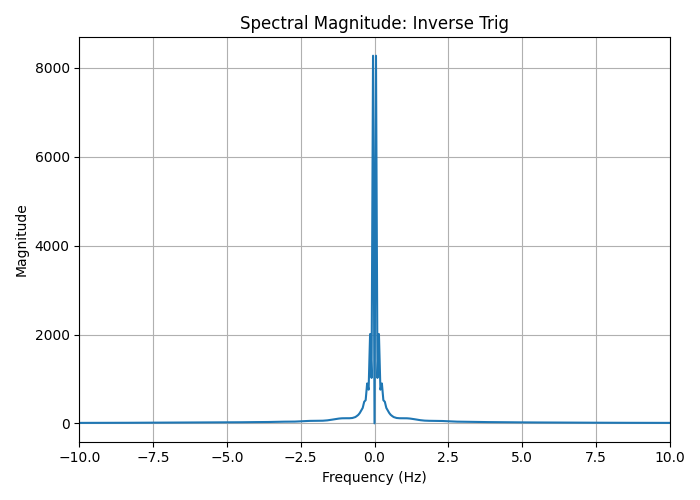
\includegraphics[height=5cm]{figs/Analysis9.png}
    \end{subfigure}
\end{figure}
Peak in spectral Analysis can be seen at frequency=0 as no oscillation
\end{document}

